\documentclass[landscape]{article}
\usepackage[utf8]{inputenc}
\usepackage[T1]{fontenc}

\usepackage[margin=1in]{geometry}
\usepackage{tikz-qtree}
\usetikzlibrary{trees}
\begin{document}
\tikzset{font=\small,
edge from parent fork down,
level distance=1.75cm,
every tree node/.style={align=center}
}

\centering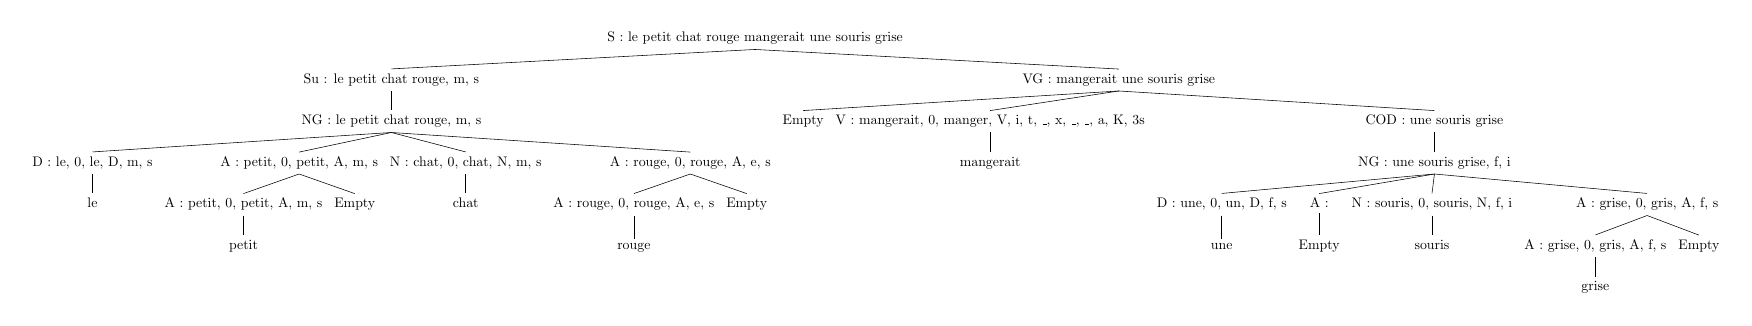
\begin{tikzpicture}[scale=0.5]
\Tree [.{S : le petit chat rouge mangerait une  souris grise \\  }
[.{Su : le petit chat rouge \\ , m, s}
[.{NG : le petit chat rouge \\ , m, s}
[.{D : le \\ , 0, le, D, m, s}
[.{le} ] ]
[.{A : petit \\ , 0, petit, A, m, s}
[.{A : petit \\ , 0, petit, A, m, s}
[.{petit} ] ]
[.{Empty} ] ]
[.{N : chat \\ , 0, chat, N, m, s}
[.{chat} ] ]
[.{A : rouge \\ , 0, rouge, A, e, s}
[.{A : rouge \\ , 0, rouge, A, e, s}
[.{rouge} ] ]
[.{Empty} ] ]
 ]
 ]
[.{VG : mangerait une  souris grise \\ }
[.{Empty} ][.{V : mangerait \\ , 0, manger, V, i, t, \_, x, \_, \_, a, K, 3s}
[.{mangerait} ] ]
[.{COD : une  souris grise \\ }
[.{NG : une  souris grise \\ , f, i}
[.{D : une \\ , 0, un, D, f, s}
[.{une} ] ]
[.{A :  \\ }
[.{Empty} ] ]
[.{N : souris \\ , 0, souris, N, f, i}
[.{souris} ] ]
[.{A : grise \\ , 0, gris, A, f, s}
[.{A : grise \\ , 0, gris, A, f, s}
[.{grise} ] ]
[.{Empty} ] ]
 ]
 ]
 ]
 ]
\end{tikzpicture}

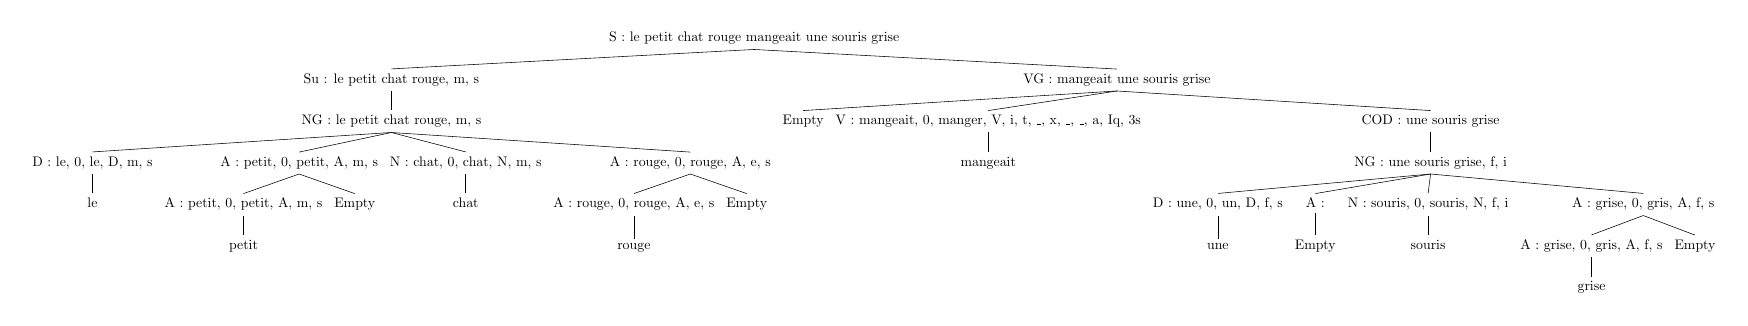
\begin{tikzpicture}[scale=0.5]
\Tree [.{S : le petit chat rouge mangeait une  souris grise \\  }
[.{Su : le petit chat rouge \\ , m, s}
[.{NG : le petit chat rouge \\ , m, s}
[.{D : le \\ , 0, le, D, m, s}
[.{le} ] ]
[.{A : petit \\ , 0, petit, A, m, s}
[.{A : petit \\ , 0, petit, A, m, s}
[.{petit} ] ]
[.{Empty} ] ]
[.{N : chat \\ , 0, chat, N, m, s}
[.{chat} ] ]
[.{A : rouge \\ , 0, rouge, A, e, s}
[.{A : rouge \\ , 0, rouge, A, e, s}
[.{rouge} ] ]
[.{Empty} ] ]
 ]
 ]
[.{VG : mangeait une  souris grise \\ }
[.{Empty} ][.{V : mangeait \\ , 0, manger, V, i, t, \_, x, \_, \_, a, Iq, 3s}
[.{mangeait} ] ]
[.{COD : une  souris grise \\ }
[.{NG : une  souris grise \\ , f, i}
[.{D : une \\ , 0, un, D, f, s}
[.{une} ] ]
[.{A :  \\ }
[.{Empty} ] ]
[.{N : souris \\ , 0, souris, N, f, i}
[.{souris} ] ]
[.{A : grise \\ , 0, gris, A, f, s}
[.{A : grise \\ , 0, gris, A, f, s}
[.{grise} ] ]
[.{Empty} ] ]
 ]
 ]
 ]
 ]
\end{tikzpicture}

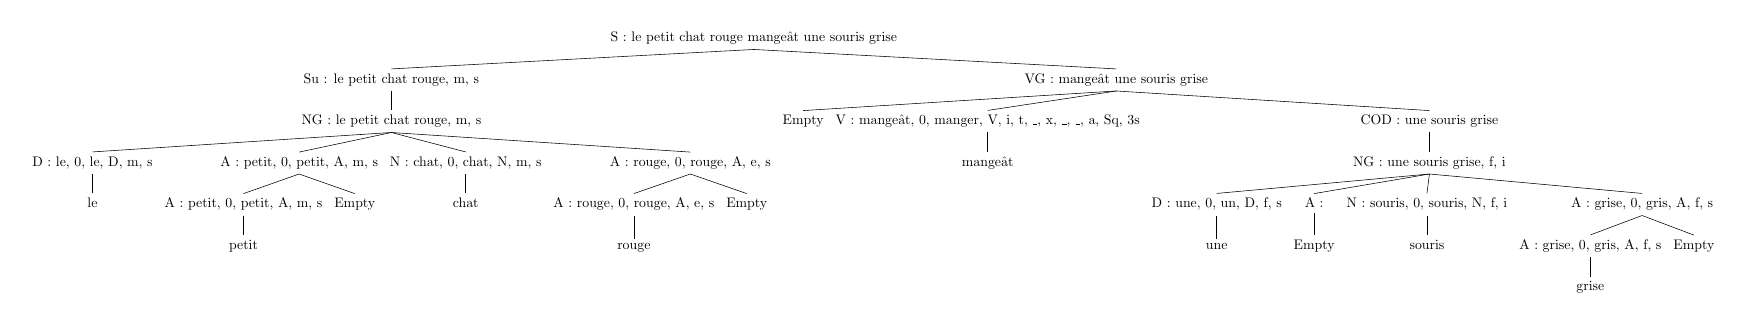
\begin{tikzpicture}[scale=0.5]
\Tree [.{S : le petit chat rouge mangeât une  souris grise \\  }
[.{Su : le petit chat rouge \\ , m, s}
[.{NG : le petit chat rouge \\ , m, s}
[.{D : le \\ , 0, le, D, m, s}
[.{le} ] ]
[.{A : petit \\ , 0, petit, A, m, s}
[.{A : petit \\ , 0, petit, A, m, s}
[.{petit} ] ]
[.{Empty} ] ]
[.{N : chat \\ , 0, chat, N, m, s}
[.{chat} ] ]
[.{A : rouge \\ , 0, rouge, A, e, s}
[.{A : rouge \\ , 0, rouge, A, e, s}
[.{rouge} ] ]
[.{Empty} ] ]
 ]
 ]
[.{VG : mangeât une  souris grise \\ }
[.{Empty} ][.{V : mangeât \\ , 0, manger, V, i, t, \_, x, \_, \_, a, Sq, 3s}
[.{mangeât} ] ]
[.{COD : une  souris grise \\ }
[.{NG : une  souris grise \\ , f, i}
[.{D : une \\ , 0, un, D, f, s}
[.{une} ] ]
[.{A :  \\ }
[.{Empty} ] ]
[.{N : souris \\ , 0, souris, N, f, i}
[.{souris} ] ]
[.{A : grise \\ , 0, gris, A, f, s}
[.{A : grise \\ , 0, gris, A, f, s}
[.{grise} ] ]
[.{Empty} ] ]
 ]
 ]
 ]
 ]
\end{tikzpicture}

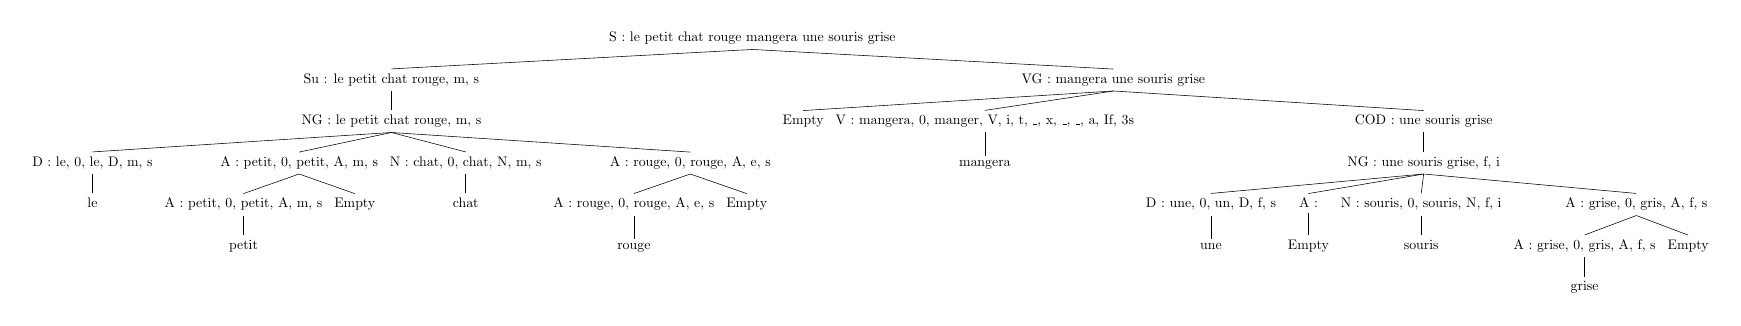
\begin{tikzpicture}[scale=0.5]
\Tree [.{S : le petit chat rouge mangera une  souris grise \\  }
[.{Su : le petit chat rouge \\ , m, s}
[.{NG : le petit chat rouge \\ , m, s}
[.{D : le \\ , 0, le, D, m, s}
[.{le} ] ]
[.{A : petit \\ , 0, petit, A, m, s}
[.{A : petit \\ , 0, petit, A, m, s}
[.{petit} ] ]
[.{Empty} ] ]
[.{N : chat \\ , 0, chat, N, m, s}
[.{chat} ] ]
[.{A : rouge \\ , 0, rouge, A, e, s}
[.{A : rouge \\ , 0, rouge, A, e, s}
[.{rouge} ] ]
[.{Empty} ] ]
 ]
 ]
[.{VG : mangera une  souris grise \\ }
[.{Empty} ][.{V : mangera \\ , 0, manger, V, i, t, \_, x, \_, \_, a, If, 3s}
[.{mangera} ] ]
[.{COD : une  souris grise \\ }
[.{NG : une  souris grise \\ , f, i}
[.{D : une \\ , 0, un, D, f, s}
[.{une} ] ]
[.{A :  \\ }
[.{Empty} ] ]
[.{N : souris \\ , 0, souris, N, f, i}
[.{souris} ] ]
[.{A : grise \\ , 0, gris, A, f, s}
[.{A : grise \\ , 0, gris, A, f, s}
[.{grise} ] ]
[.{Empty} ] ]
 ]
 ]
 ]
 ]
\end{tikzpicture}

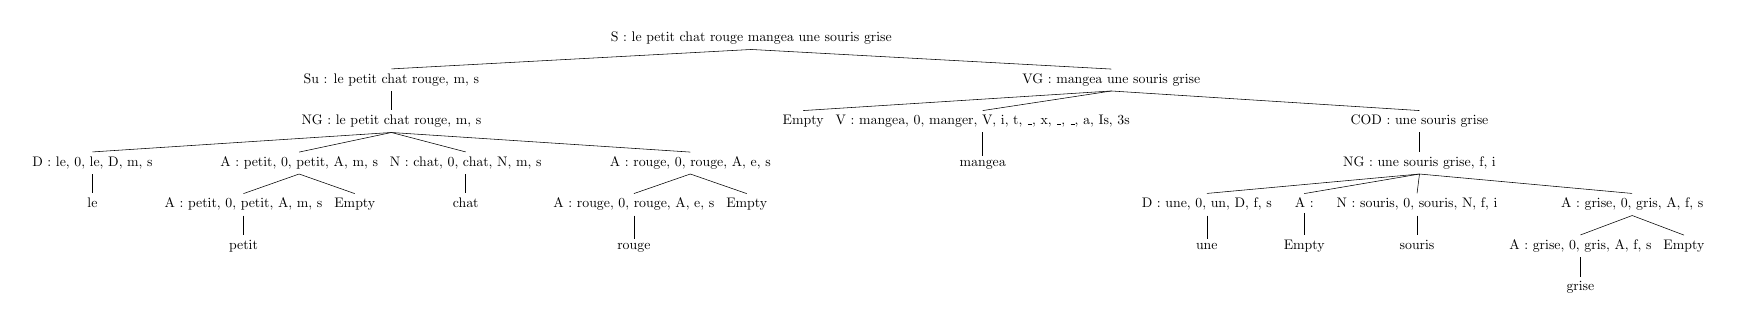
\begin{tikzpicture}[scale=0.5]
\Tree [.{S : le petit chat rouge mangea une  souris grise \\  }
[.{Su : le petit chat rouge \\ , m, s}
[.{NG : le petit chat rouge \\ , m, s}
[.{D : le \\ , 0, le, D, m, s}
[.{le} ] ]
[.{A : petit \\ , 0, petit, A, m, s}
[.{A : petit \\ , 0, petit, A, m, s}
[.{petit} ] ]
[.{Empty} ] ]
[.{N : chat \\ , 0, chat, N, m, s}
[.{chat} ] ]
[.{A : rouge \\ , 0, rouge, A, e, s}
[.{A : rouge \\ , 0, rouge, A, e, s}
[.{rouge} ] ]
[.{Empty} ] ]
 ]
 ]
[.{VG : mangea une  souris grise \\ }
[.{Empty} ][.{V : mangea \\ , 0, manger, V, i, t, \_, x, \_, \_, a, Is, 3s}
[.{mangea} ] ]
[.{COD : une  souris grise \\ }
[.{NG : une  souris grise \\ , f, i}
[.{D : une \\ , 0, un, D, f, s}
[.{une} ] ]
[.{A :  \\ }
[.{Empty} ] ]
[.{N : souris \\ , 0, souris, N, f, i}
[.{souris} ] ]
[.{A : grise \\ , 0, gris, A, f, s}
[.{A : grise \\ , 0, gris, A, f, s}
[.{grise} ] ]
[.{Empty} ] ]
 ]
 ]
 ]
 ]
\end{tikzpicture}

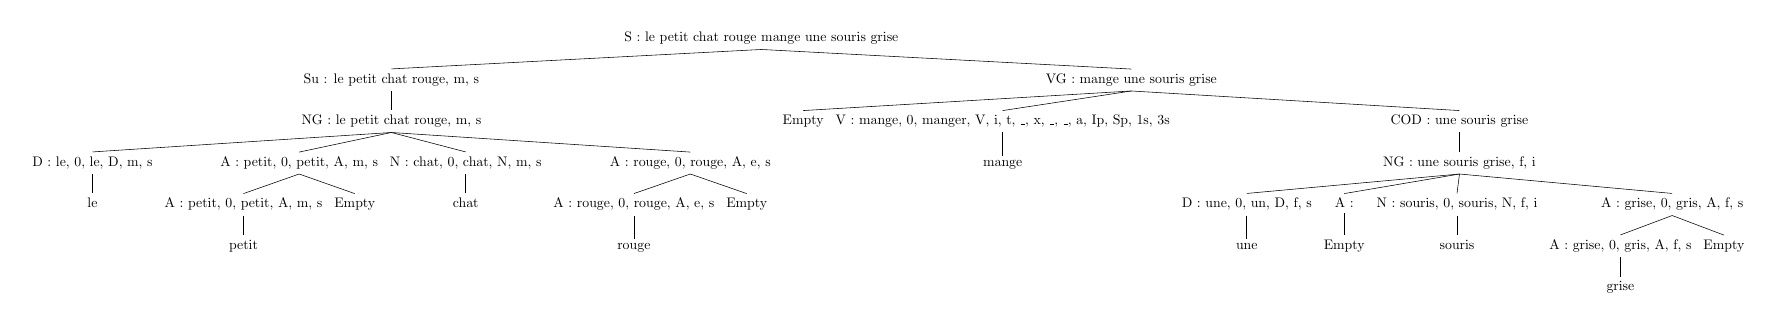
\begin{tikzpicture}[scale=0.5]
\Tree [.{S : le petit chat rouge mange une  souris grise \\  }
[.{Su : le petit chat rouge \\ , m, s}
[.{NG : le petit chat rouge \\ , m, s}
[.{D : le \\ , 0, le, D, m, s}
[.{le} ] ]
[.{A : petit \\ , 0, petit, A, m, s}
[.{A : petit \\ , 0, petit, A, m, s}
[.{petit} ] ]
[.{Empty} ] ]
[.{N : chat \\ , 0, chat, N, m, s}
[.{chat} ] ]
[.{A : rouge \\ , 0, rouge, A, e, s}
[.{A : rouge \\ , 0, rouge, A, e, s}
[.{rouge} ] ]
[.{Empty} ] ]
 ]
 ]
[.{VG : mange une  souris grise \\ }
[.{Empty} ][.{V : mange \\ , 0, manger, V, i, t, \_, x, \_, \_, a, Ip, Sp, 1s, 3s}
[.{mange} ] ]
[.{COD : une  souris grise \\ }
[.{NG : une  souris grise \\ , f, i}
[.{D : une \\ , 0, un, D, f, s}
[.{une} ] ]
[.{A :  \\ }
[.{Empty} ] ]
[.{N : souris \\ , 0, souris, N, f, i}
[.{souris} ] ]
[.{A : grise \\ , 0, gris, A, f, s}
[.{A : grise \\ , 0, gris, A, f, s}
[.{grise} ] ]
[.{Empty} ] ]
 ]
 ]
 ]
 ]
\end{tikzpicture}

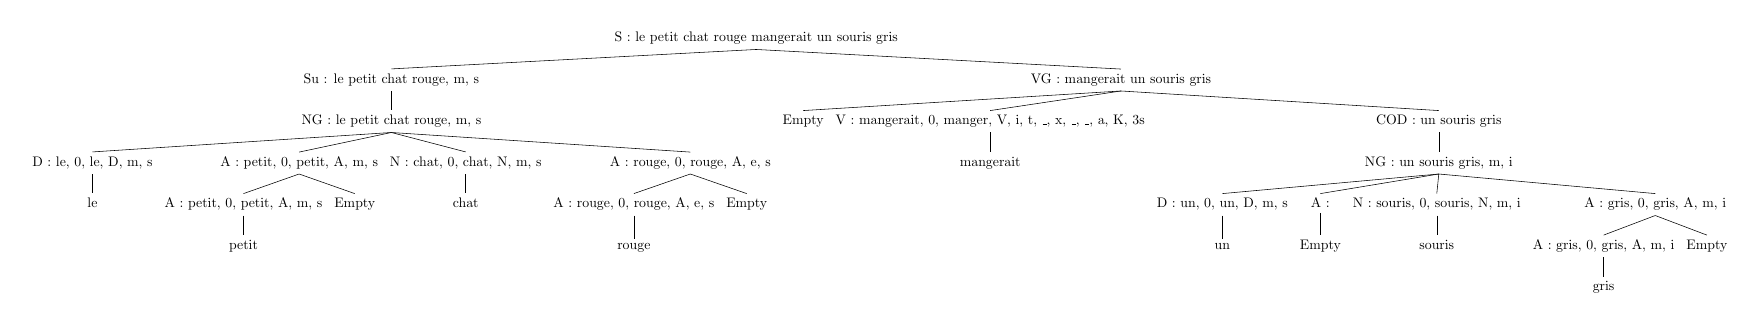
\begin{tikzpicture}[scale=0.5]
\Tree [.{S : le petit chat rouge mangerait un  souris gris \\  }
[.{Su : le petit chat rouge \\ , m, s}
[.{NG : le petit chat rouge \\ , m, s}
[.{D : le \\ , 0, le, D, m, s}
[.{le} ] ]
[.{A : petit \\ , 0, petit, A, m, s}
[.{A : petit \\ , 0, petit, A, m, s}
[.{petit} ] ]
[.{Empty} ] ]
[.{N : chat \\ , 0, chat, N, m, s}
[.{chat} ] ]
[.{A : rouge \\ , 0, rouge, A, e, s}
[.{A : rouge \\ , 0, rouge, A, e, s}
[.{rouge} ] ]
[.{Empty} ] ]
 ]
 ]
[.{VG : mangerait un  souris gris \\ }
[.{Empty} ][.{V : mangerait \\ , 0, manger, V, i, t, \_, x, \_, \_, a, K, 3s}
[.{mangerait} ] ]
[.{COD : un  souris gris \\ }
[.{NG : un  souris gris \\ , m, i}
[.{D : un \\ , 0, un, D, m, s}
[.{un} ] ]
[.{A :  \\ }
[.{Empty} ] ]
[.{N : souris \\ , 0, souris, N, m, i}
[.{souris} ] ]
[.{A : gris \\ , 0, gris, A, m, i}
[.{A : gris \\ , 0, gris, A, m, i}
[.{gris} ] ]
[.{Empty} ] ]
 ]
 ]
 ]
 ]
\end{tikzpicture}

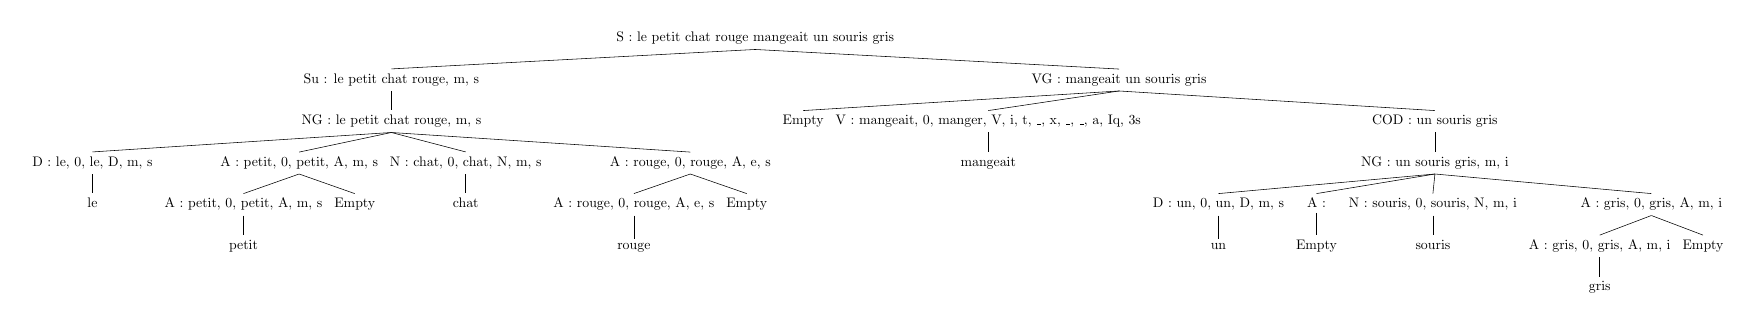
\begin{tikzpicture}[scale=0.5]
\Tree [.{S : le petit chat rouge mangeait un  souris gris \\  }
[.{Su : le petit chat rouge \\ , m, s}
[.{NG : le petit chat rouge \\ , m, s}
[.{D : le \\ , 0, le, D, m, s}
[.{le} ] ]
[.{A : petit \\ , 0, petit, A, m, s}
[.{A : petit \\ , 0, petit, A, m, s}
[.{petit} ] ]
[.{Empty} ] ]
[.{N : chat \\ , 0, chat, N, m, s}
[.{chat} ] ]
[.{A : rouge \\ , 0, rouge, A, e, s}
[.{A : rouge \\ , 0, rouge, A, e, s}
[.{rouge} ] ]
[.{Empty} ] ]
 ]
 ]
[.{VG : mangeait un  souris gris \\ }
[.{Empty} ][.{V : mangeait \\ , 0, manger, V, i, t, \_, x, \_, \_, a, Iq, 3s}
[.{mangeait} ] ]
[.{COD : un  souris gris \\ }
[.{NG : un  souris gris \\ , m, i}
[.{D : un \\ , 0, un, D, m, s}
[.{un} ] ]
[.{A :  \\ }
[.{Empty} ] ]
[.{N : souris \\ , 0, souris, N, m, i}
[.{souris} ] ]
[.{A : gris \\ , 0, gris, A, m, i}
[.{A : gris \\ , 0, gris, A, m, i}
[.{gris} ] ]
[.{Empty} ] ]
 ]
 ]
 ]
 ]
\end{tikzpicture}

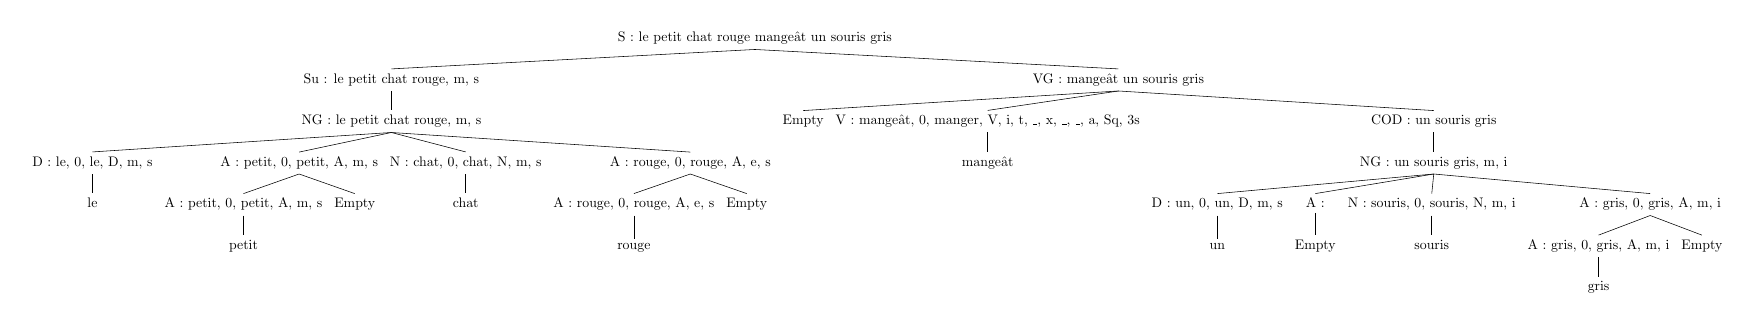
\begin{tikzpicture}[scale=0.5]
\Tree [.{S : le petit chat rouge mangeât un  souris gris \\  }
[.{Su : le petit chat rouge \\ , m, s}
[.{NG : le petit chat rouge \\ , m, s}
[.{D : le \\ , 0, le, D, m, s}
[.{le} ] ]
[.{A : petit \\ , 0, petit, A, m, s}
[.{A : petit \\ , 0, petit, A, m, s}
[.{petit} ] ]
[.{Empty} ] ]
[.{N : chat \\ , 0, chat, N, m, s}
[.{chat} ] ]
[.{A : rouge \\ , 0, rouge, A, e, s}
[.{A : rouge \\ , 0, rouge, A, e, s}
[.{rouge} ] ]
[.{Empty} ] ]
 ]
 ]
[.{VG : mangeât un  souris gris \\ }
[.{Empty} ][.{V : mangeât \\ , 0, manger, V, i, t, \_, x, \_, \_, a, Sq, 3s}
[.{mangeât} ] ]
[.{COD : un  souris gris \\ }
[.{NG : un  souris gris \\ , m, i}
[.{D : un \\ , 0, un, D, m, s}
[.{un} ] ]
[.{A :  \\ }
[.{Empty} ] ]
[.{N : souris \\ , 0, souris, N, m, i}
[.{souris} ] ]
[.{A : gris \\ , 0, gris, A, m, i}
[.{A : gris \\ , 0, gris, A, m, i}
[.{gris} ] ]
[.{Empty} ] ]
 ]
 ]
 ]
 ]
\end{tikzpicture}

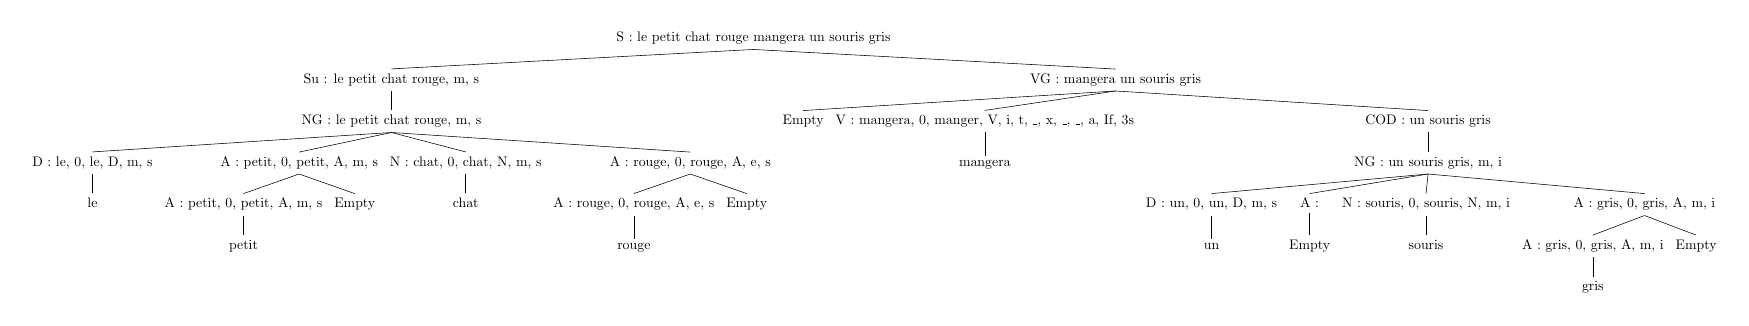
\begin{tikzpicture}[scale=0.5]
\Tree [.{S : le petit chat rouge mangera un  souris gris \\  }
[.{Su : le petit chat rouge \\ , m, s}
[.{NG : le petit chat rouge \\ , m, s}
[.{D : le \\ , 0, le, D, m, s}
[.{le} ] ]
[.{A : petit \\ , 0, petit, A, m, s}
[.{A : petit \\ , 0, petit, A, m, s}
[.{petit} ] ]
[.{Empty} ] ]
[.{N : chat \\ , 0, chat, N, m, s}
[.{chat} ] ]
[.{A : rouge \\ , 0, rouge, A, e, s}
[.{A : rouge \\ , 0, rouge, A, e, s}
[.{rouge} ] ]
[.{Empty} ] ]
 ]
 ]
[.{VG : mangera un  souris gris \\ }
[.{Empty} ][.{V : mangera \\ , 0, manger, V, i, t, \_, x, \_, \_, a, If, 3s}
[.{mangera} ] ]
[.{COD : un  souris gris \\ }
[.{NG : un  souris gris \\ , m, i}
[.{D : un \\ , 0, un, D, m, s}
[.{un} ] ]
[.{A :  \\ }
[.{Empty} ] ]
[.{N : souris \\ , 0, souris, N, m, i}
[.{souris} ] ]
[.{A : gris \\ , 0, gris, A, m, i}
[.{A : gris \\ , 0, gris, A, m, i}
[.{gris} ] ]
[.{Empty} ] ]
 ]
 ]
 ]
 ]
\end{tikzpicture}

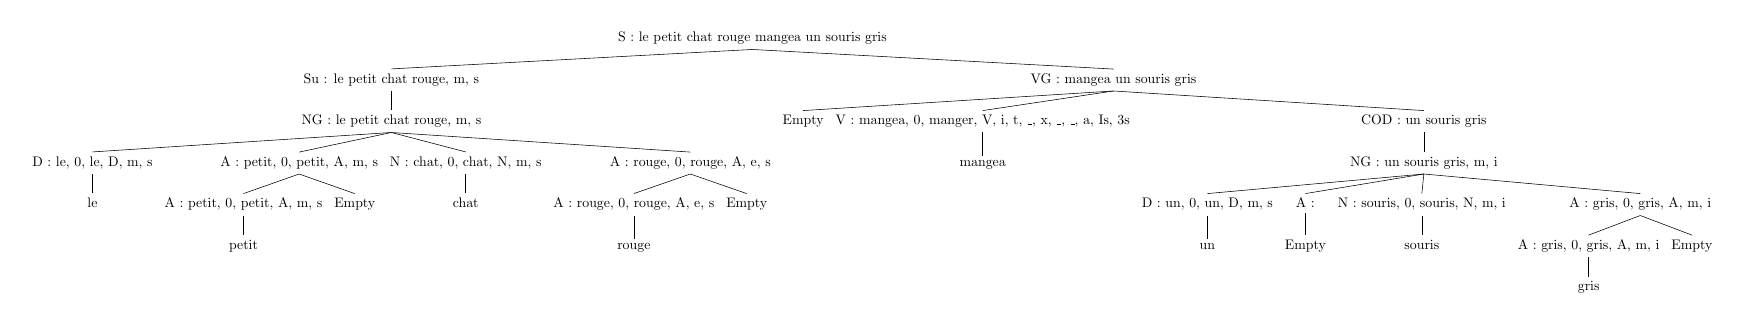
\begin{tikzpicture}[scale=0.5]
\Tree [.{S : le petit chat rouge mangea un  souris gris \\  }
[.{Su : le petit chat rouge \\ , m, s}
[.{NG : le petit chat rouge \\ , m, s}
[.{D : le \\ , 0, le, D, m, s}
[.{le} ] ]
[.{A : petit \\ , 0, petit, A, m, s}
[.{A : petit \\ , 0, petit, A, m, s}
[.{petit} ] ]
[.{Empty} ] ]
[.{N : chat \\ , 0, chat, N, m, s}
[.{chat} ] ]
[.{A : rouge \\ , 0, rouge, A, e, s}
[.{A : rouge \\ , 0, rouge, A, e, s}
[.{rouge} ] ]
[.{Empty} ] ]
 ]
 ]
[.{VG : mangea un  souris gris \\ }
[.{Empty} ][.{V : mangea \\ , 0, manger, V, i, t, \_, x, \_, \_, a, Is, 3s}
[.{mangea} ] ]
[.{COD : un  souris gris \\ }
[.{NG : un  souris gris \\ , m, i}
[.{D : un \\ , 0, un, D, m, s}
[.{un} ] ]
[.{A :  \\ }
[.{Empty} ] ]
[.{N : souris \\ , 0, souris, N, m, i}
[.{souris} ] ]
[.{A : gris \\ , 0, gris, A, m, i}
[.{A : gris \\ , 0, gris, A, m, i}
[.{gris} ] ]
[.{Empty} ] ]
 ]
 ]
 ]
 ]
\end{tikzpicture}

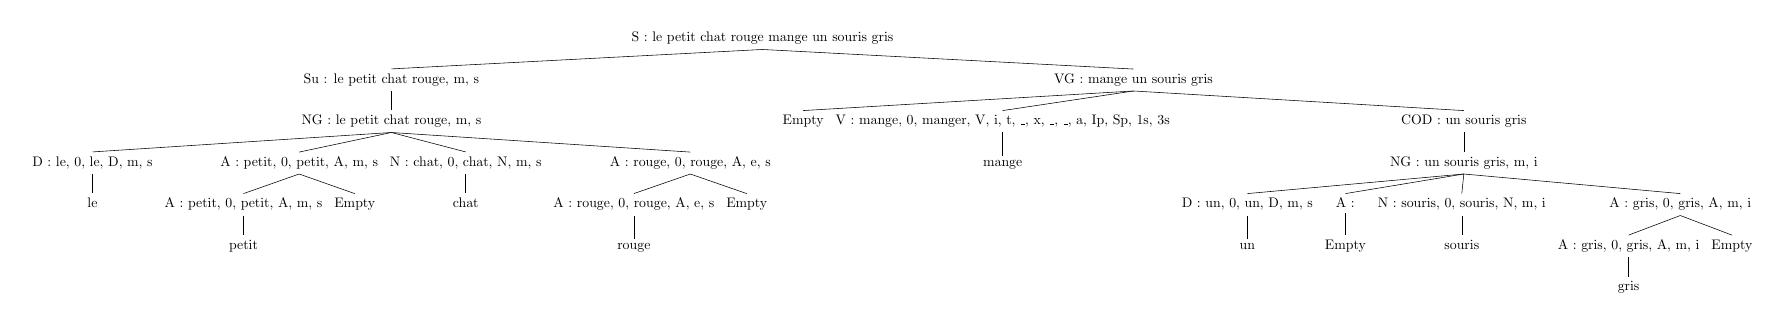
\begin{tikzpicture}[scale=0.5]
\Tree [.{S : le petit chat rouge mange un  souris gris \\  }
[.{Su : le petit chat rouge \\ , m, s}
[.{NG : le petit chat rouge \\ , m, s}
[.{D : le \\ , 0, le, D, m, s}
[.{le} ] ]
[.{A : petit \\ , 0, petit, A, m, s}
[.{A : petit \\ , 0, petit, A, m, s}
[.{petit} ] ]
[.{Empty} ] ]
[.{N : chat \\ , 0, chat, N, m, s}
[.{chat} ] ]
[.{A : rouge \\ , 0, rouge, A, e, s}
[.{A : rouge \\ , 0, rouge, A, e, s}
[.{rouge} ] ]
[.{Empty} ] ]
 ]
 ]
[.{VG : mange un  souris gris \\ }
[.{Empty} ][.{V : mange \\ , 0, manger, V, i, t, \_, x, \_, \_, a, Ip, Sp, 1s, 3s}
[.{mange} ] ]
[.{COD : un  souris gris \\ }
[.{NG : un  souris gris \\ , m, i}
[.{D : un \\ , 0, un, D, m, s}
[.{un} ] ]
[.{A :  \\ }
[.{Empty} ] ]
[.{N : souris \\ , 0, souris, N, m, i}
[.{souris} ] ]
[.{A : gris \\ , 0, gris, A, m, i}
[.{A : gris \\ , 0, gris, A, m, i}
[.{gris} ] ]
[.{Empty} ] ]
 ]
 ]
 ]
 ]
\end{tikzpicture}

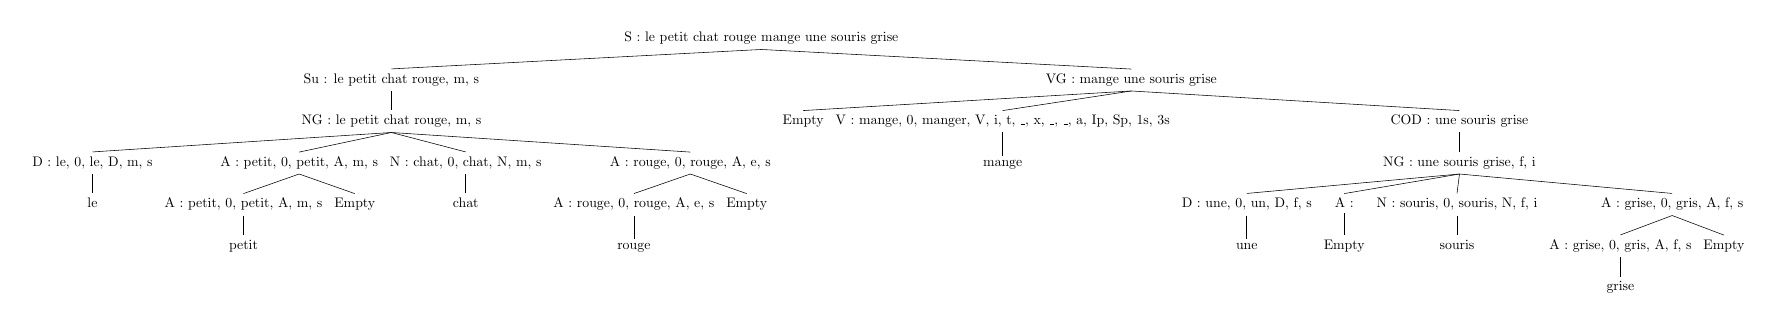
\begin{tikzpicture}[scale=0.5]
\Tree [.{S : le petit chat rouge mange une  souris grise \\  }
[.{Su : le petit chat rouge \\ , m, s}
[.{NG : le petit chat rouge \\ , m, s}
[.{D : le \\ , 0, le, D, m, s}
[.{le} ] ]
[.{A : petit \\ , 0, petit, A, m, s}
[.{A : petit \\ , 0, petit, A, m, s}
[.{petit} ] ]
[.{Empty} ] ]
[.{N : chat \\ , 0, chat, N, m, s}
[.{chat} ] ]
[.{A : rouge \\ , 0, rouge, A, e, s}
[.{A : rouge \\ , 0, rouge, A, e, s}
[.{rouge} ] ]
[.{Empty} ] ]
 ]
 ]
[.{VG : mange une  souris grise \\ }
[.{Empty} ][.{V : mange \\ , 0, manger, V, i, t, \_, x, \_, \_, a, Ip, Sp, 1s, 3s}
[.{mange} ] ]
[.{COD : une  souris grise \\ }
[.{NG : une  souris grise \\ , f, i}
[.{D : une \\ , 0, un, D, f, s}
[.{une} ] ]
[.{A :  \\ }
[.{Empty} ] ]
[.{N : souris \\ , 0, souris, N, f, i}
[.{souris} ] ]
[.{A : grise \\ , 0, gris, A, f, s}
[.{A : grise \\ , 0, gris, A, f, s}
[.{grise} ] ]
[.{Empty} ] ]
 ]
 ]
 ]
 ]
\end{tikzpicture}

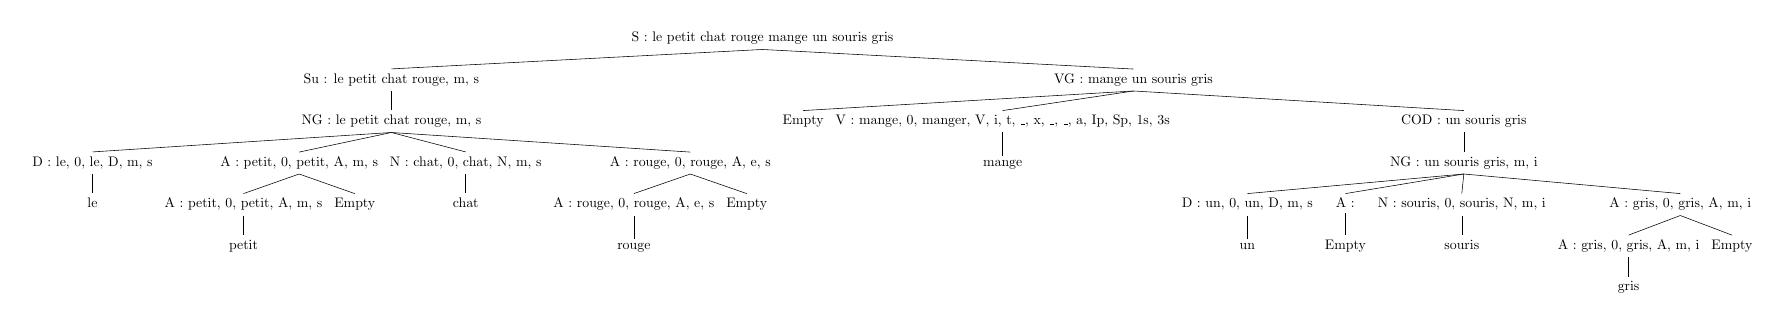
\begin{tikzpicture}[scale=0.5]
\Tree [.{S : le petit chat rouge mange un  souris gris \\  }
[.{Su : le petit chat rouge \\ , m, s}
[.{NG : le petit chat rouge \\ , m, s}
[.{D : le \\ , 0, le, D, m, s}
[.{le} ] ]
[.{A : petit \\ , 0, petit, A, m, s}
[.{A : petit \\ , 0, petit, A, m, s}
[.{petit} ] ]
[.{Empty} ] ]
[.{N : chat \\ , 0, chat, N, m, s}
[.{chat} ] ]
[.{A : rouge \\ , 0, rouge, A, e, s}
[.{A : rouge \\ , 0, rouge, A, e, s}
[.{rouge} ] ]
[.{Empty} ] ]
 ]
 ]
[.{VG : mange un  souris gris \\ }
[.{Empty} ][.{V : mange \\ , 0, manger, V, i, t, \_, x, \_, \_, a, Ip, Sp, 1s, 3s}
[.{mange} ] ]
[.{COD : un  souris gris \\ }
[.{NG : un  souris gris \\ , m, i}
[.{D : un \\ , 0, un, D, m, s}
[.{un} ] ]
[.{A :  \\ }
[.{Empty} ] ]
[.{N : souris \\ , 0, souris, N, m, i}
[.{souris} ] ]
[.{A : gris \\ , 0, gris, A, m, i}
[.{A : gris \\ , 0, gris, A, m, i}
[.{gris} ] ]
[.{Empty} ] ]
 ]
 ]
 ]
 ]
\end{tikzpicture}


\end{document}
